\subsubsection{Aufgabe der Komponente}
Über die WiFi-Direct Komponente vermitteln die Peers ihre Kontaktdaten an alle ver\-füg\-ba\-ren Peers in der Nähe. Dies geschieht über den Expose Befehl des ASIP Protokolls, bei dem ein ASIP-Interesse an die Wissensbasis von anderen Peers gesandt wird. Dies beinhaltet unter anderem die Bluetooth MAC-Adresse, mit der dem Peer dann anschließend Nachrichten per Bluetooth geschickt werden können. Das Verschicken der Bluetooth Mac-Adresse via WiFi-Direct ermöglicht es daher, dass für die darauf folgende Bluetooth-Verbindung kein Pairing benötigt wird. 
\\Die Komponente ist der elementare Bestandteil des Peer-Radars, der alle sich in der Nähe befindlichen Peers anzeigt und die Kommunikation mit diesen erlaubt. Das Radar ist wiederum dafür erforderlich, neue Chats mit Peers anzulegen oder einen semantischen Broadcast ohne Bluetooth-Pairing zu ermöglichen.


\subsubsection{Architektur}

\subsubsubsection{Überlick}\label{ch:wifioverview}

Im folgenden UML-Klassendiagramm sind alle Bestandteile der WiFi-Direct Komponente von SharkNet abgebildet.
\begin{figure}[H]
	\centering
	\hspace*{1cm}
	\makebox[\linewidth][c]{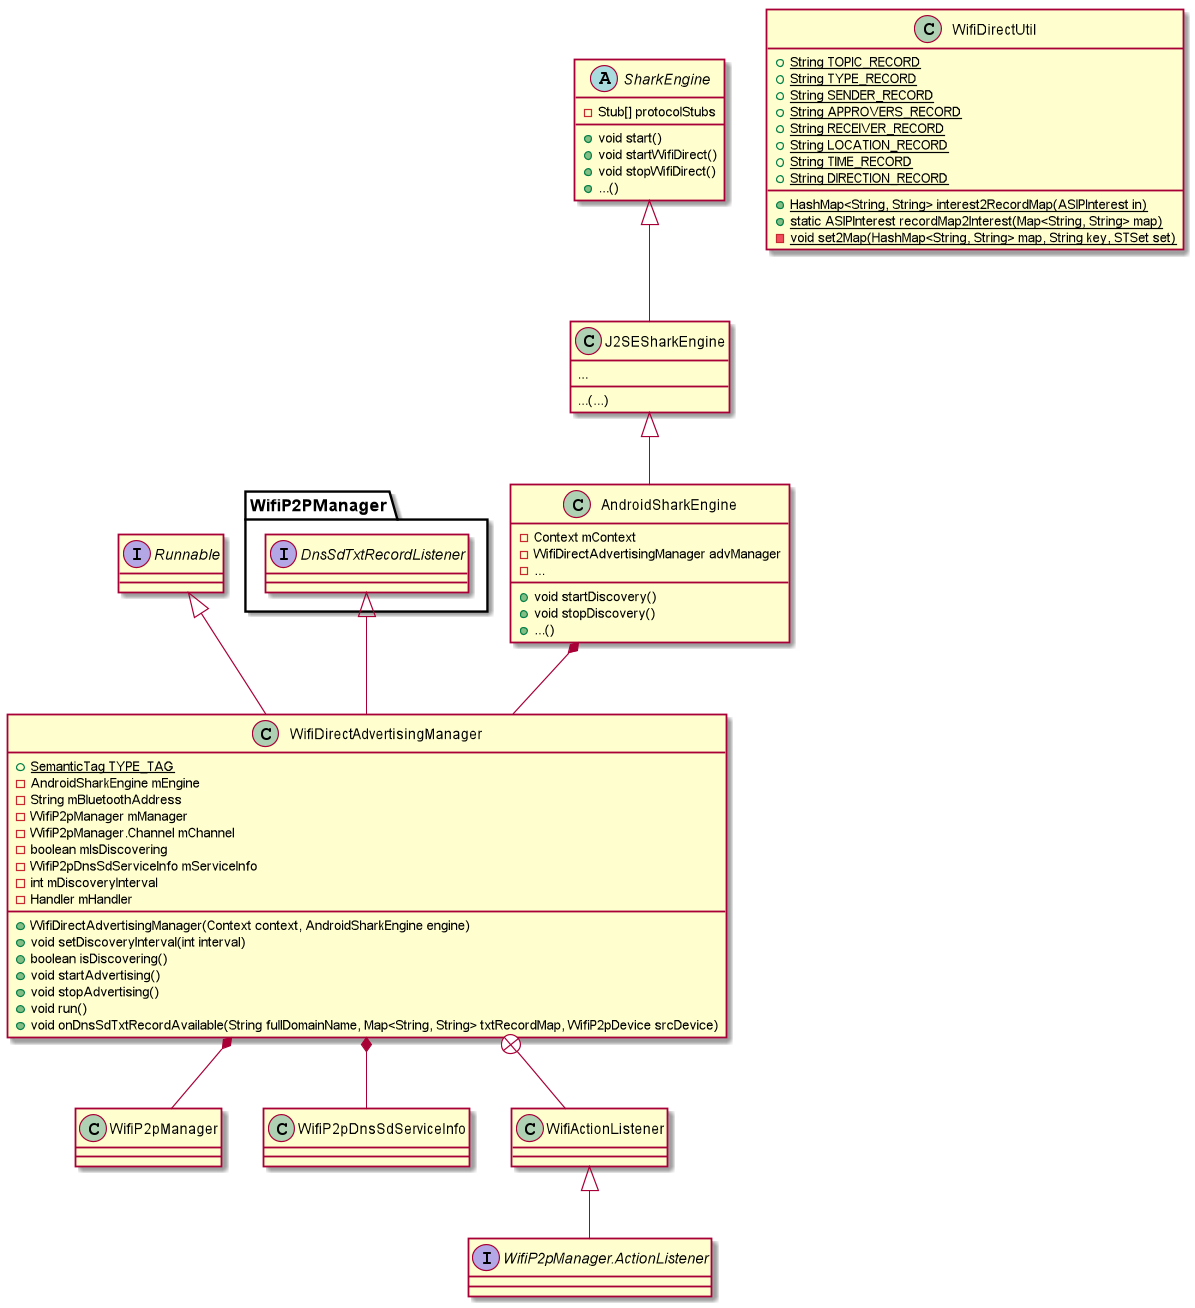
\includegraphics[width=1.1\linewidth]{wifi/images/wifiDirectGesamt.png}}%
	\caption{Die WiFi-Direct Klassen im Überblick}
	\label{fig:wifiAll}
\end{figure}
Im Zentrum dieser Hierarchie steht die Klasse \textit{WiFiDirectAdvertisingManager}. Eine Instanz dieser Klasse befindet sich als Attribut in der Klasse \textit{AndroidSharkEngine}, von der aus alle Protokolle wie NFC, Wifi-Direct oder Bluetooth gesteuert werden. Über die Engine kann daher auch das Radar per \textit{startDiscovery()} Methode gestartet oder über die \textit{stopDiscovery()} Methode beendet werden. Das Starten oder Stoppen der kompletten WiFi-Komponente erfolgt dagegen in der Klasse \textit{AndroidSharkEngine}, die den Ausgangspunkt der Vererbungshierarchie darstellt.
\\Die Klasse \textit{WifiDirectUtil} bietet statische Methoden an, mit denen ASIP-Interessen in Hashmaps umgewandelt werden können und umgekehrt. Dies ist notwendig, da die von Android gestellte Basisklasse \textit{WifiP2PManager} bei der Anmeldungen von Services keine ASIP-Interessen, sondern Hashmaps als Parameter akzeptiert.

\subsubsection{Nutzung}
Die WiFi-Komponente wird automatisch beim Start der Anwendung gestartet. Manuell kann die Komponente über die Klasse \textit{AndroidSharkEngine} gesteuert werden, welche wie schon im Überblick erwähnt die beiden Methoden \textit{startDiscovery()} und \textit{stopDiscovery()} enthält.


\subsubsubsection{Code}
Der Code dieser Komponente kann hier \url{https://github.com/SharedKnowledge/SharkNet-Api-Android/tree/master/api/src/main/java/net/sharksystem/api/shark/protocols/wifidirect} betrachtet werden. Wie auch die anderen Implementierungen von Übertragungsprotokollen, befindet sich auch die WiFi-Direct-Implementierung im Projekt \textit{SharkNet-Api-Android} im Package \textit{protocols}.
\\Wie im vorherigen Unterkapitel erläutert liefern die beiden Methoden \textit{startDiscovery()} und \textit{stopDiscovery()} die Funktionalität, um Peers zu finden und andere Peers über das eigene Interesse in Kenntnis zu setzen. 
\\Bei Aufruf der \textit{startDiscovery()} Methode wird innerhalb der Engine ein neuer \textit{WifiDirectAdvertisingManager} angelegt und anschließend dessen \textit{startAdvertising()} Methode aufgerufen. Innerhalb der \textit{startAdvertising()} Methode wird sich nun auf der dritten Schicht des OSI-Modells begeben, wie der folgende Codeausschnitt zeigt:
\lstset{language=Java, caption=Hinzufügung des Services, label=DescriptiveLabel, numbers=left, numbersep=1em, breaklines=true, basicstyle=\small}
\begin{lstlisting}
HashMap<String, String> map = WifiDirectUtil.interest2RecordMap(interest);
mServiceInfo = WifiP2pDnsSdServiceInfo.newInstance("_sbc", "_presence._tcp", map);
mManager.addLocalService(mChannel, mServiceInfo, new WifiActionListener("Add LocalService"));
mManager.clearServiceRequests(mChannel, new WifiActionListener("Clear ServiceRequests"));
WifiP2pDnsSdServiceRequest wifiP2pDnsSdServiceRequest = WifiP2pDnsSdServiceRequest.newInstance();
mManager.addServiceRequest(mChannel, wifiP2pDnsSdServiceRequest, new WifiActionListener("Add ServiceRequest"));
\end{lstlisting}
Nachdem in der erste Zeile eine Hashmap auf dem Interesse erzeugt worden ist, wird diese Hashmap in Zeile zwei als Parameter für die Erzeugung einer Service Information benutzt. Anschließend wird dem \textit{WifiP2PManager} ein neuer lokaler Service hinzugefügt, wobei dieser Service die zuvor erzeugte Service Information enthält. Nachdem etwaige vorherige Service Requests beseitigt worden sind, wird der neue WifiP2P Service Request hinzugefügt. Dadurch wird nun an alle Geräte in der Nähe, die auf WifiP2P Service Requests warten, dieser zur Verfügung gestellt.
\\Neben dem Hinzufügen von Services, müssen diese aber auch empfangen und ausgewertet werden. Dies ist der Grund, warum der \textit{WifiDirectAdvertisingManager} das Interface \textit{Runnable} implementiert. In der dadurch implementierten Methode \textit{run()} werden die von anderen Geräten gesendeten Service Requests empfangen.
\lstset{language=Java, caption=Erkennung von Services, label=DescriptiveLabel, numbers=left, numbersep=1em, breaklines=true, basicstyle=\small}
\begin{lstlisting}
mManager.discoverServices(mChannel, new WifiActionListener("Discover Services"));
mHandler.postDelayed(this, mDiscoveryInterval);
\end{lstlisting}
Sollte ein Service gefunden und erfolgreich eine Peer-To-Peer Verbindung zwischen zwei Geräten aufgebaut werden können, wird nun die aus Listing x.x bekannte Hashmap an das Gerät gesendet, welches den Service gefunden (discovered) hat. Dabei wird automatisch die Methode \textit{onDnsSdTxtRecordAvailable} aufgerufen, welche die empfangene Hashmap in ein ASIP-Interesse umwandelt und dann der Engine weiterreicht.
\lstset{language=Java, caption=Vewertung des Interesses, label=DescriptiveLabel, numbers=left, numbersep=1em, breaklines=true, basicstyle=\small}
\begin{lstlisting}
ASIPInterest interest = WifiDirectUtil.recordMap2Interest(txtRecordMap);
mEngine.handleASIPInterest(interest);
\end{lstlisting}  

\subsubsubsection{Deployment / Runtime}
lorem ipsum


\subsubsection{Test}
\subsubsubsection{Gerätetest}
Mit den folgenden Android-Geräten ist die Komponente auf Kompatibilität geprüft worden:
\begin{table}[H]
	\begin{center}
		\caption{Kompatibilitätstest der Komponente}
		\label{tab:dimensions}
		\begin{tabular}{l|c|c} 			
			Gerät & Android-Version & kompatibel \\
			\hline
			LG Nexus 5x & 8.0 & Ja\\
			LG Nexus 5x & 8.1 & Ja\\
			LG Nexus 5 & 6.1 & Ja\\
			Sony Xperia XZ Premium & 8.0 & Ja\\
			Sony Xperia Z4 Tablet & 7.1.1 & Ja\\
			Lenovo B & 6.0 & Ja\\
			Lenovo A5500-F Tablet & 4.4 & Nein\\
			Raspberry Pi 3 & 6.0.1 & Nein\\	
			Wandboard Quad & 5.0.2 & Nein\\			
		\end{tabular}
	\end{center}
\end{table}
Die beiden Einplatinencomputer Raspberry Pi 3 und Wandboard Quad unterstützen zwar grundsätzlich WLAN, jedoch nicht WiFi-Direct. Beim Raspberry Pi 3 wäre WiFi-Direct zwar technisch möglich, benötigt aber zahlreiche Umkonfigurationen, was dadurch dann nicht mehr eine reine Android-Version darstellt. 
\\Das Lenovo A5500-F Tablet hat mit Android 4.4 eine zu alte Version, die nicht alle von der Komponente benötigten WiFi-Direct Klassen bereitstellt. 
\\Nach dem Update des LG Nexus 5x von Android 8.0 auf die Version 8.1 ist zu beachten, dass das Gerät seine Bluetooth MAC-Adresse nicht mehr programmatisch auslesen kann. Dies betrifft vor allem die Bluetooth-Komponente und wird in der dazugehörigen Komponentenbeschreibung vertieft.  

\subsubsection{Ausblick}
Die WiFi Komponente wurde SharkNet hinzugefügt, da der wiederholte Austausch von Kontakdaten zwischen den Geräten mit Bluetooth zu viel Zeit in Anspruch genommen hat. Da jedes Gerät standardmäßig alle zehn Sekunden seine Anmeldedaten an Geräte in der Nähe schickt, musste diese eher ungewöhnliche Aufteilung erfolgen. Wenn zukünftig die Bluetooth-Komponente auf Bluetooth Low Energy umgestellt werden sollte, ist es eventuell möglich, auf die WiFi Komponente zu verzichten und den gesamten Datenaustausch über Bluetooth vorzunehmen. 
\newpage